\documentclass{standalone}

\usepackage{tikz}
\usepackage{amssymb}
\usetikzlibrary{calc, positioning}
\begin{document}
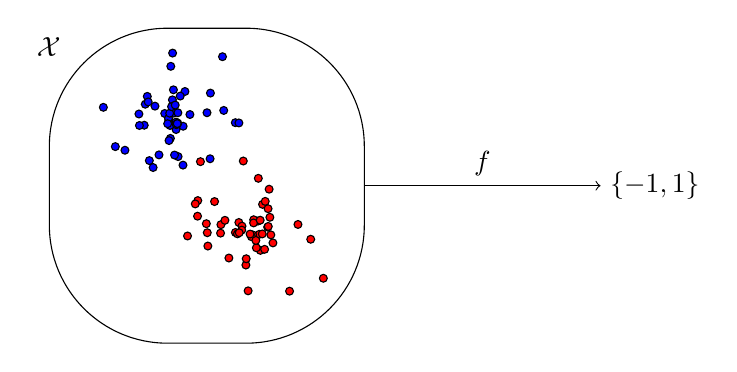
\begin{tikzpicture}
	\pgfmathsetseed{1}
	\draw[rounded corners = 1.5cm] (-2,-2) -- (-2,2) -- (2,2) -- (2,-2) -- cycle;
	\coordinate (x) at (2,0);
	\node[below] at (current bounding box.north west) {$ \mathcal{X} $};

	\begin{scope}[shift={(-0.4,0.8)}]
		\foreach \x in {1,...,50}{
				\filldraw[fill=blue] ({rnd*rand}, {rnd*rand}) circle (0.05);
			}
	\end{scope}

	\begin{scope}[shift={(0.6,-0.6)}]
		\foreach \x in {1,...,50}{
				\filldraw[fill=red] ({rnd*rand}, {rnd*rand}) circle (0.05);
			}
	\end{scope}


	\begin{scope}[xshift=5cm]
		\coordinate[label={right:$ \{ -1,1 \} $}] (y) at (0,0);
	\end{scope}

	\draw[->] (x) -- node[midway, above] {$ f $} (y);

\end{tikzpicture}
\end{document}
